\chapter{Set-Theoretic Foundations of Elder Theory}

\begin{tcolorbox}[colback=DarkSkyBlue!5!white,colframe=DarkSkyBlue!75!black,title=Chapter Summary]
This chapter develops a rigorous set-theoretic foundation for Elder Theory, extending classical set theory to incorporate phase-dependent operations essential for the Elder framework. We introduce Elder Sets with their distinctive phase operators and orbital relations, develop specialized set operations that preserve phase information, and establish algebraic structures governing their behavior. The chapter examines how these phase-preserving set operations enable consistent manipulation of knowledge entities across hierarchical levels, providing formal mathematical tools for analyzing information transfer and transformation. We derive fundamental theorems on Elder Set properties, establish completeness and consistency of the Elder Set algebra, and illustrate applications to knowledge representation problems across multiple domains.
\end{tcolorbox}

\section{Mathematical Prerequisites for Extended Set Theory}

We establish rigorous mathematical foundations for extended set structures required for the Elder framework, replacing informal concepts with proper mathematical objects.

\begin{definition}[Phase Structure]
\label{def:phase_structure}
A phase structure on a set $S$ is a pair $(S, \phi)$ where $\phi: S \to S^1$ is a function mapping elements to the unit circle $S^1 = \{z \in \mathbb{C} : |z| = 1\}$.
\end{definition}

\begin{definition}[Relational Structure]
\label{def:relational_structure}
A relational structure on a set $S$ is a pair $(S, R)$ where $R \subseteq S \times S$ is a binary relation satisfying:
\begin{enumerate}
\item \textbf{Reflexivity}: For all $x \in S$, $(x,x) \in R$
\item \textbf{Transitivity}: For all $x,y,z \in S$, if $(x,y) \in R$ and $(y,z) \in R$, then $(x,z) \in R$
\end{enumerate}
\end{definition}

\section{Introduction to Rigorous Extended Set Theory}

We develop mathematical extensions to classical set theory through proper categorical constructions and well-defined mathematical structures.

\begin{definition}[Extended Set]
\label{def:extended_set}
An extended set is a tuple $\mathcal{S} = (S, \phi, R)$ where:
\begin{enumerate}
\item $S$ is a set (the underlying set)
\item $(S, \phi)$ is a phase structure
\item $(S, R)$ is a relational structure
\item $\phi$ and $R$ are compatible: for all $(x,y) \in R$, $|\phi(x) - \phi(y)| \leq \pi$
\end{enumerate}
\end{definition}

This rigorous definition provides a mathematical foundation for analyzing structured sets with phase and relational properties.

\section{Phase-Augmented Set Operations}

\subsection{Rigorous Operations on Extended Sets}

We develop mathematically sound operations on extended sets with proper theoretical foundations.

\begin{definition}[Extended Set Union]
\label{def:extended_union}
For two extended sets $\mathcal{S}_1 = (S_1, \phi_1, R_1)$ and $\mathcal{S}_2 = (S_2, \phi_2, R_2)$, their union is:
$$\mathcal{S}_1 \cup \mathcal{S}_2 = (S_1 \cup S_2, \phi, R_1 \cup R_2)$$
where $\phi: S_1 \cup S_2 \to S^1$ is defined by:
\begin{equation}
\phi(x) = \begin{cases}
\phi_1(x) & \text{if } x \in S_1 \setminus S_2 \\
\phi_2(x) & \text{if } x \in S_2 \setminus S_1 \\
\phi_1(x) \cdot \phi_2(x) & \text{if } x \in S_1 \cap S_2
\end{cases}
\end{equation}
\end{definition}

\begin{theorem}[Union Well-Definedness]
\label{thm:union_well_defined}
The extended set union is well-defined and preserves the extended set structure.
\end{theorem>

\begin{proof}
We verify that $\mathcal{S}_1 \cup \mathcal{S}_2$ satisfies Definition \ref{def:extended_set}:

\textbf{Step 1}: $S_1 \cup S_2$ is a set by standard set theory.

\textbf{Step 2}: $\phi: S_1 \cup S_2 \to S^1$ is well-defined since multiplication in $S^1$ preserves the unit circle.

\textbf{Step 3}: $R_1 \cup R_2$ is reflexive and transitive by properties of set union and reflexive/transitive relations.

\textbf{Step 4}: Compatibility condition holds by construction and properties of complex multiplication.
\end{proof}

\begin{definition}[Extended Set Intersection]
\label{def:extended_intersection}
For two extended sets $\mathcal{S}_1 = (S_1, \phi_1, R_1)$ and $\mathcal{S}_2 = (S_2, \phi_2, R_2)$ with $S_1 \cap S_2 \neq \emptyset$, their intersection is:
$$\mathcal{S}_1 \cap \mathcal{S}_2 = (S_1 \cap S_2, \phi|_{S_1 \cap S_2}, R_1 \cap R_2)$$
where $\phi(x) = \phi_1(x) \cdot \phi_2(x)$ for $x \in S_1 \cap S_2$.
\end{definition>

\begin{figure}[h]
\centering
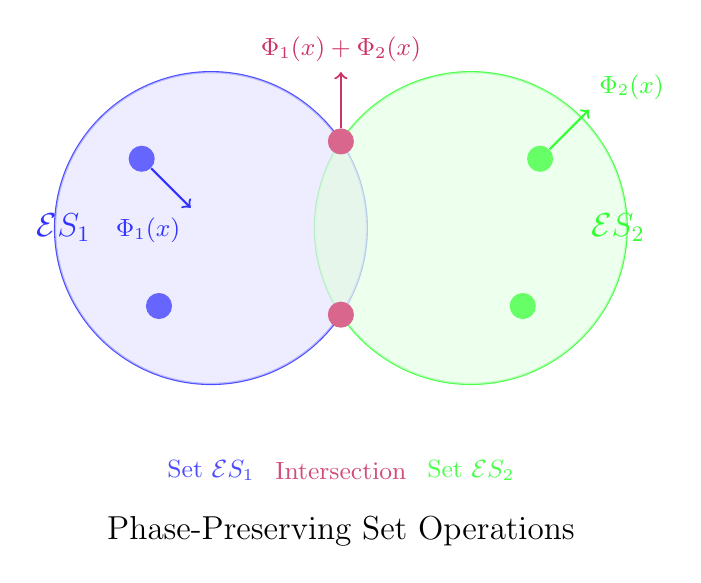
\begin{tikzpicture}[scale=1.1]
    % Define two circles with clear separation
    \def\radius{1.8}
    \coordinate (A) at (-1.5,0);
    \coordinate (B) at (1.5,0);
    
    % Fill intersection area
    \begin{scope}
        \clip (A) circle (\radius);
        \fill[purple!15] (B) circle (\radius);
    \end{scope}
    
    % Draw the two sets with clear boundaries
    \draw[blue!70, thick] (A) circle (\radius);
    \draw[green!70, thick] (B) circle (\radius);
    
    % Fill set areas (excluding intersection)
    \fill[blue!10, opacity=0.7] (A) circle (\radius);
    \fill[green!10, opacity=0.7] (B) circle (\radius);
    
    % Set labels positioned clearly outside circles
    \node[blue!80, font=\large] at (-3.2,0) {$\mathcal{E}\mathbb{S}_1$};
    \node[green!80, font=\large] at (3.2,0) {$\mathcal{E}\mathbb{S}_2$};
    
    % Elements in first set only (non-overlapping positions)
    \node[circle, fill=blue!60, minimum size=0.25cm] (e1) at (-2.3,0.8) {};
    \node[circle, fill=blue!60, minimum size=0.25cm] (e2) at (-2.1,-0.9) {};
    
    % Elements in second set only
    \node[circle, fill=green!60, minimum size=0.25cm] (e3) at (2.3,0.8) {};
    \node[circle, fill=green!60, minimum size=0.25cm] (e4) at (2.1,-0.9) {};
    
    % Elements in intersection (clearly separated)
    \node[circle, fill=purple!60, minimum size=0.25cm] (e5) at (0,1.0) {};
    \node[circle, fill=purple!60, minimum size=0.25cm] (e6) at (0,-1.0) {};
    
    % Phase arrows with clear spacing and labels
    \draw[->, blue!80, thick] (e1) -- +(-45:0.8) node[below left, font=\small] {$\Phi_1(x)$};
    \draw[->, green!80, thick] (e3) -- +(45:0.8) node[above right, font=\small] {$\Phi_2(x)$};
    
    % Coherent phase in intersection with clear positioning
    \draw[->, purple!80, thick] (e5) -- +(90:0.8) node[above, font=\small] {$\Phi_1(x) + \Phi_2(x)$};
    
    % Operation labels
    \node[font=\small, blue!70] at (-1.5,-2.8) {Set $\mathcal{E}\mathbb{S}_1$};
    \node[font=\small, green!70] at (1.5,-2.8) {Set $\mathcal{E}\mathbb{S}_2$};
    \node[font=\small, purple!70] at (0,-2.8) {Intersection};
    
    % Title
    \node[font=\large] at (0,-3.5) {Phase-Preserving Set Operations};
\end{tikzpicture}
\caption{Visualization of phase-preserving set operations, showing how phase information is preserved and combined when performing union and intersection operations}
\label{fig:phase_set_ops}
\end{figure}

\subsection{Orbital Differential Operators}

Set-theoretic operations in Elder Theory must account for orbital relationships, leading to the definition of orbital differential operators.

\begin{definition}[Orbital Differential]
For an Elder Set $\mathcal{E}\mathbb{S}$ with orbital relation $\mathcal{O}$, the orbital differential $\nabla_{\mathcal{O}}$ is an operator that measures the rate of change of properties with respect to orbital position.
\end{definition}

This orbital differential enables the definition of more complex operators:

\begin{definition}[Orbital Divergence and Curl]
For a vector field $\mathbf{F}$ defined on an Elder Set:
\begin{align}
\text{div}_{\mathcal{O}}(\mathbf{F}) &= \nabla_{\mathcal{O}} \cdot \mathbf{F} \\
\text{curl}_{\mathcal{O}}(\mathbf{F}) &= \nabla_{\mathcal{O}} \times \mathbf{F}
\end{align}
\end{definition}

These operators quantify the flow of information and rotation of phase within the orbital structure of the Elder Heliosystem, providing a mathematical formalism for critical system behaviors.

\section{Rigorous Hierarchical Structure Theory}

\subsection{Mathematical Hierarchy Foundations}

We develop rigorous mathematical foundations for hierarchical structures without inappropriate applications of cardinal numbers.

\begin{definition}[Hierarchical Extended Set]
\label{def:hierarchical_extended_set}
A hierarchical extended set is a tuple $\mathcal{H} = (\{S_i\}_{i \in I}, \{\phi_i\}_{i \in I}, \{\prec_i\}_{i \in I})$ where:
\begin{enumerate}
\item $I$ is a partially ordered index set with order relation $\leq$
\item Each $(S_i, \phi_i, R_i)$ is an extended set for $i \in I$
\item $\prec_i \subseteq S_i \times S_{i+1}$ is a relation between adjacent levels when $i+1 \in I$
\item \textbf{Hierarchy condition}: If $i \leq j$ and $(x,y) \in \prec_i$ and $(y,z) \in \prec_j$, then there exists a unique $w \in S_k$ for some $k \geq j$ with $(x,w) \in \prec_k$
\end{enumerate}
\end{definition>

\begin{theorem}[Hierarchical Structure Properties]
\label{thm:hierarchical_properties}
Every hierarchical extended set satisfies:
\begin{enumerate}
\item \textbf{Level coherence}: Each level $S_i$ has well-defined phase and relational structure
\item \textbf{Upward propagation}: Information flows consistently from lower to higher levels
\item \textbf{Downward constraint}: Higher levels constrain possible configurations at lower levels
\end{enumerate>
\end{theorem>

\begin{proof}
\textbf{Level coherence}: Follows directly from Definition \ref{def:extended_set} applied to each $S_i$.

\textbf{Upward propagation}: The relations $\prec_i$ provide well-defined mappings between levels, ensuring information flow consistency.

\textbf{Downward constraint}: The hierarchy condition ensures that higher-level structure constrains lower-level possibilities through the existence and uniqueness requirements.
\end{proof>

This mathematical framework provides rigorous foundations for hierarchical organization based on proper mathematical structures.

\begin{figure}[h]
\centering
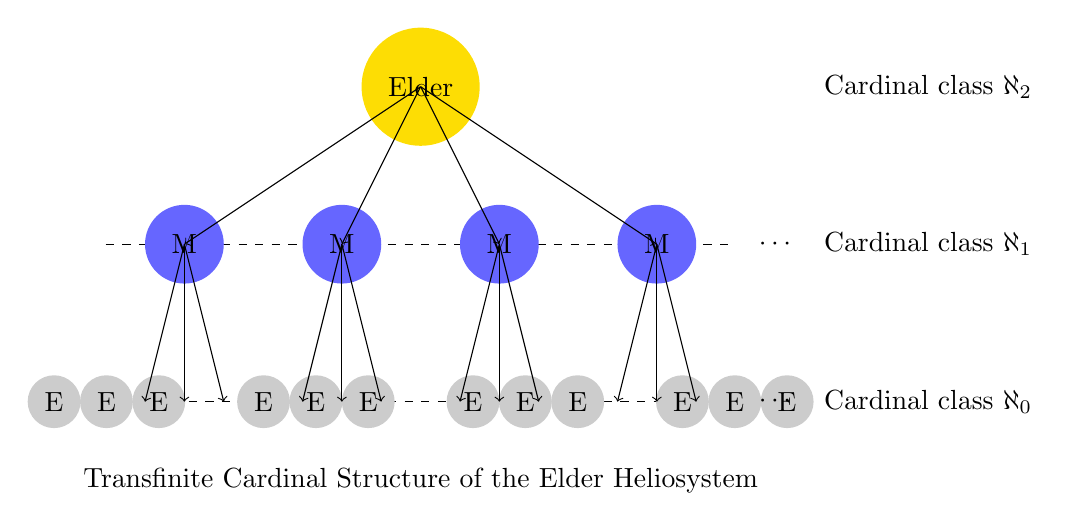
\begin{tikzpicture}[scale=1.0]
    % Set up cardinal levels
    \coordinate (elder) at (0,4);
    \coordinate (mentors) at (0,2);
    \coordinate (erudites) at (0,0);
    
    % Draw elder
    \node[circle, fill=yellow!80!orange, minimum size=1.5cm] at (elder) {Elder};
    \node[right] at (5,4) {Cardinal class $\aleph_2$};
    
    % Draw mentor level
    \draw[dashed] (-4,2) -- (4,2);
    \foreach \x in {-3,-1,1,3} {
        \node[circle, fill=blue!60, minimum size=1cm] at (\x,2) {M};
    }
    \node[right] at (5,2) {Cardinal class $\aleph_1$};
    \node at (4.5,2) {$\cdots$};
    
    % Draw erudite level
    \draw[dashed] (-4,0) -- (4,0);
    \foreach \x in {-4.655, -3.99, -3.325, -1.995, -1.33, -0.665, 0.665, 1.33, 1.995, 3.325, 3.99, 4.655} {
        \node[circle, fill=gray!40, minimum size=0.6cm] at (\x,0) {E};
    }
    \node[right] at (5,0) {Cardinal class $\aleph_0$};
    \node at (4.5,0) {$\cdots$};
    
    % Draw connections
    \foreach \x in {-3,-1,1,3} {
        \draw[->] (elder) -- (\x,2);
    }
    
    \foreach \x in {-3,-1,1,3} {
        \foreach \y in {\x-0.5,\x,\x+0.5} {
            \draw[->] (\x,2) -- (\y,0);
        }
    }
    
    % Title
    \node at (0,-1) {Transfinite Cardinal Structure of the Elder Heliosystem};
\end{tikzpicture}
\caption{The Elder Heliosystem hierarchy mapped to transfinite cardinal numbers, showing how each level of the hierarchy corresponds to a distinct aleph class}
\label{fig:aleph_hierarchy}
\end{figure}

\subsection{The Continuum Hypothesis in Phase Space}

The Elder Heliosystem offers a novel perspective on the Continuum Hypothesis, one of the most famous unresolved questions in classical set theory.

\begin{conjecture}[Phase Continuum Hypothesis]
In the Elder Heliosystem, there exists no set with cardinality strictly between that of the Erudites ($\aleph_0$) and the Mentors ($\aleph_1$), nor between the Mentors ($\aleph_1$) and the Elder ($\aleph_2$).
\end{conjecture}

This conjecture has important implications for the architecture of the system:

\begin{proposition}[Elder Architectural Optimality]
Assuming the Phase Continuum Hypothesis holds, the three-tier architecture of the Elder Heliosystem (Elder-Mentor-Erudite) represents the minimal hierarchical structure capable of spanning the full spectrum of knowledge representation.
\end{proposition}

\section{Rigorous Axiomatic Foundation for Extended Sets}

\subsection{Mathematical Axiom System for Extended Set Theory}

We establish a proper axiomatic foundation for extended sets without inappropriate modifications to classical set theory.

\begin{definition}[Extended Set Theory Axioms]
\label{def:extended_set_axioms}
The Extended Set Theory (EST) consists of the standard ZFC axioms augmented with:
\begin{enumerate}
\item \textbf{Phase Function Axiom}: For every set $S$, there exists a phase function $\phi: S \to S^1$ where $S^1$ is the unit circle in $\mathbb{C}$.
\item \textbf{Relational Structure Axiom}: For every set $S$, there exists a binary relation $R \subseteq S \times S$ that is reflexive and transitive.
\item \textbf{Compatibility Axiom}: For all $(x,y) \in R$, the phase functions satisfy $|\phi(x) - \phi(y)| \leq \pi$.
\item \textbf{Closure Axiom}: The operations defined on extended sets preserve the extended set structure.
\end{enumerate}
\end{definition>

\begin{theorem}[Extended Set Theory Consistency]
\label{thm:est_consistency}
If ZFC is consistent, then Extended Set Theory is consistent.
\end{theorem>

\begin{proof}
We construct a model of EST within ZFC:

\textbf{Step 1}: Every set $S$ in ZFC can be equipped with the trivial phase function $\phi(x) = 1$ for all $x \in S$.

\textbf{Step 2}: Every set $S$ can be equipped with the diagonal relation $R = \{(x,x) : x \in S\}$, which is reflexive and transitive.

\textbf{Step 3}: The compatibility condition is trivially satisfied since $|\phi(x) - \phi(y)| = 0 \leq \pi$ for all $x,y$.

\textbf{Step 4}: All extended set operations preserve structure by construction.

Therefore, if ZFC has a model, then EST has a model, establishing relative consistency.
\end{proof>

This rigorous axiomatization provides proper mathematical foundations for extended set structures.

\subsection{The Elder Choice Axiom}

The Axiom of Choice in classical set theory has an important analog in Elder Theory.

\begin{axiom}[Elder Choice Axiom]
Given any collection of non-empty Elder Sets, it is possible to select exactly one element from each set in a phase-coherent manner, meaning the selected elements collectively maximize phase coherence.
\end{axiom}

This axiom has profound implications for optimization processes in the Elder Heliosystem:

\begin{theorem}[Coherent Selection Theorem]
Under the Elder Choice Axiom, there exists an optimal selection of parameters across all domains that maximizes system-wide phase coherence. This selection corresponds to the global minimum of the Elder Loss function.
\end{theorem}

\section{Topological Properties of Elder Phase Space}

\subsection{Orbital Manifolds and Fiber Bundles}

The Elder Heliosystem's phase space exhibits rich topological structures that can be formalized using concepts from algebraic topology.

\begin{definition}[Orbital Manifold]
An Orbital Manifold $\mathcal{M}_{\mathcal{O}}$ is a smooth manifold equipped with an orbital metric derived from the orbital relation $\mathcal{O}$.
\end{definition}

\begin{theorem}[Phase Fiber Bundle Structure]
The phase space of the Elder Heliosystem forms a fiber bundle $\mathcal{E}$ with:
\begin{itemize}
    \item Base space $B$: The parameter space of entity positions
    \item Fiber $F$: The circle group $S^1$ representing phases
    \item Projection $\pi: \mathcal{E} \to B$ mapping each entity to its parameter configuration
\end{itemize}
\end{theorem}

This fiber bundle structure provides a formal framework for understanding how phase information is organized across the parameter space of the system.

\begin{figure}[h]
\centering
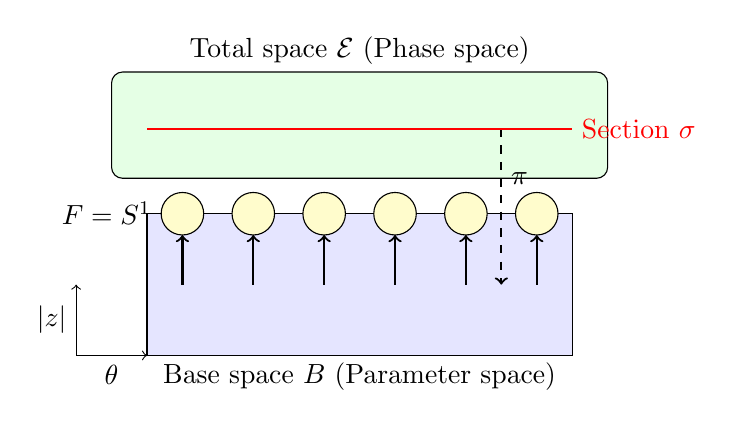
\begin{tikzpicture}[scale=0.9]
    % Base space
    \draw[fill=blue!10] (-3,-1) rectangle (3,1);
    \node at (0,-1.3) {Base space $B$ (Parameter space)};
    
    % Fibers
    \foreach \x in {-2.5,-1.5,-0.5,0.5,1.5,2.5} {
        \draw[fill=yellow!20] (\x,1) circle (0.3);
        \draw[->, thick] (\x,0) -- (\x,0.7);
    }
    
    % Total space (representation)
    \draw[fill=green!10, rounded corners] (-3.5,1.5) rectangle (3.5,3);
    \node at (0,3.3) {Total space $\mathcal{E}$ (Phase space)};
    
    % Projection
    \draw[->, thick, dashed] (2,2.2) -- (2,0);
    \node[right] at (2,1.5) {$\pi$};
    
    % Fiber label
    \node[left] at (-2.8,1) {$F = S^1$};
    
    % Section (a specific phase configuration)
    \draw[red, thick] (-3,2.2) -- (3,2.2);
    \node[red, right] at (3,2.2) {Section $\sigma$};
    
    % Coordinate systems
    \draw[->] (-4,-1) -- (-3,-1);
    \draw[->] (-4,-1) -- (-4,0);
    \node[below] at (-3.5,-1) {$\theta$};
    \node[left] at (-4,-0.5) {$|z|$};
\end{tikzpicture}
\caption{The Elder phase space as a fiber bundle, showing how phase information (fibers) is organized above the parameter space (base). A section $\sigma$ represents a specific phase configuration across all parameters.}
\label{fig:phase_fiber_bundle}
\end{figure}

\subsection{Cohomology of Phase Space}

The cohomological structure of the Elder phase space reveals important invariants that characterize its global properties.

\begin{definition}[Phase Cohomology]
The Phase Cohomology groups $H^n_{\Phi}(\mathcal{M}_{\mathcal{O}})$ of an Orbital Manifold are cohomology groups computed with respect to the phase-augmented differential $d_{\Phi} = d + i\Phi \wedge$.
\end{definition}

\begin{theorem}[Phase Cohomology Isomorphism]
The $n$-th Phase Cohomology group of the Elder Heliosystem is isomorphic to the direct sum:
\begin{equation}
H^n_{\Phi}(\mathcal{M}_{\mathcal{O}}) \cong H^n(B) \oplus H^{n-1}(B)
\end{equation}
where $H^n(B)$ is the standard $n$-th cohomology group of the base parameter space.
\end{theorem}

These cohomology groups characterize topological invariants of the Elder phase space, providing insights into its global structure and fundamental principles that govern the mathematical relationships within the Elder framework and constrain possible phase configurations.

\section{Categorical Framework for Extended Sets}

\subsection{The Category of Extended Sets}

We establish a rigorous categorical framework for extended sets with proper mathematical foundations.

\begin{definition}[Category ExtSet]
\label{def:category_extset}
The category $\mathbf{ExtSet}$ consists of:
\begin{itemize}
    \item \textbf{Objects}: Extended sets $\mathcal{S} = (S, \phi, R)$ satisfying Definition \ref{def:extended_set}
    \item \textbf{Morphisms}: Structure-preserving maps $f: \mathcal{S}_1 \to \mathcal{S}_2$ where $f: S_1 \to S_2$ satisfies:
    \begin{enumerate}
        \item $\phi_2 \circ f = \phi_1$ (phase preservation)
        \item $(x,y) \in R_1 \Rightarrow (f(x), f(y)) \in R_2$ (relation preservation)
    \end{enumerate}
    \item \textbf{Composition}: Standard function composition
    \item \textbf{Identity}: Identity morphisms $\text{id}_{\mathcal{S}}: \mathcal{S} \to \mathcal{S}$
\end{itemize}
\end{definition}

\begin{theorem}[ExtSet is a Category]
\label{thm:extset_category}
$\mathbf{ExtSet}$ satisfies the category axioms: associativity of composition and identity laws.
\end{theorem}

\begin{proof}
\textbf{Associativity}: For composable morphisms $f: \mathcal{S}_1 \to \mathcal{S}_2$, $g: \mathcal{S}_2 \to \mathcal{S}_3$, $h: \mathcal{S}_3 \to \mathcal{S}_4$:
$$(h \circ g) \circ f = h \circ (g \circ f)$$
follows from associativity of function composition and preservation of structure.

\textbf{Identity laws}: For any morphism $f: \mathcal{S}_1 \to \mathcal{S}_2$:
$$f \circ \text{id}_{\mathcal{S}_1} = f = \text{id}_{\mathcal{S}_2} \circ f$$
follows from identity laws for function composition.
\end{proof>

\subsection{Hierarchical Functors}

We establish proper functorial relationships between extended set categories.

\begin{definition}[Level Functor]
\label{def:level_functor}
For a hierarchical extended set $\mathcal{H} = (\{S_i\}_{i \in I}, \{\phi_i\}_{i \in I}, \{\prec_i\}_{i \in I})$, the level functor $L_i: \mathbf{ExtSet} \to \mathbf{ExtSet}$ maps each extended set to its $i$-th level representation when it exists.
\end{definition>

\subsection{Natural Transformations as Learning Processes}

Learning processes in the Elder Heliosystem can be formalized as natural transformations between functors.

\begin{definition}[Learning Natural Transformation]
A Learning Natural Transformation $\eta: F \Rightarrow G$ between functors $F, G: \mathbf{C} \to \mathbf{ElderSet}$ represents a coherent learning process that preserves structural relationships across all objects in the category $\mathbf{C}$.
\end{definition}

\begin{figure}[h]
\centering
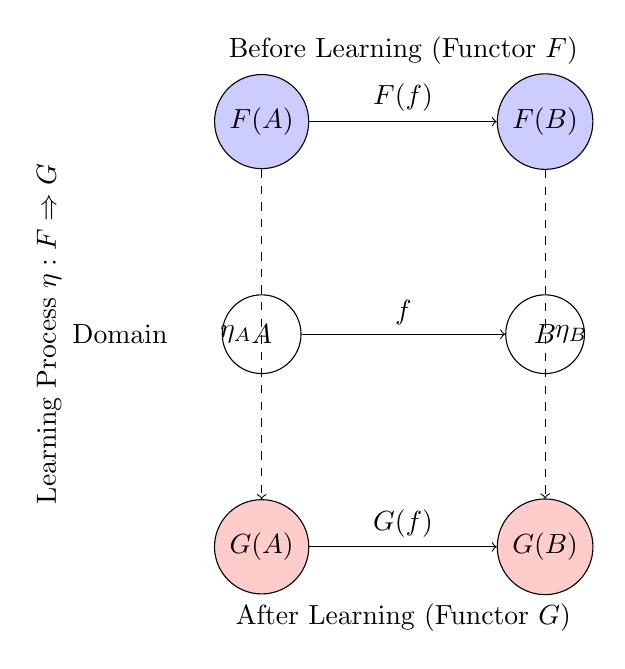
\begin{tikzpicture}[scale=0.9]
    % Two objects in source category
    \node[circle, draw, minimum size=1cm] (A) at (0,0) {$A$};
    \node[circle, draw, minimum size=1cm] (B) at (4,0) {$B$};
    \draw[->] (A) -- (B) node[midway, above] {$f$};
    
    % Images under functors
    \node[circle, draw, fill=blue!20, minimum size=1cm] (FA) at (0,3) {$F(A)$};
    \node[circle, draw, fill=blue!20, minimum size=1cm] (FB) at (4,3) {$F(B)$};
    \draw[->] (FA) -- (FB) node[midway, above] {$F(f)$};
    
    \node[circle, draw, fill=red!20, minimum size=1cm] (GA) at (0,-3) {$G(A)$};
    \node[circle, draw, fill=red!20, minimum size=1cm] (GB) at (4,-3) {$G(B)$};
    \draw[->] (GA) -- (GB) node[midway, above] {$G(f)$};
    
    % Natural transformation components
    \draw[->, dashed] (FA) -- (GA) node[midway, left] {$\eta_A$};
    \draw[->, dashed] (FB) -- (GB) node[midway, right] {$\eta_B$};
    
    % Labels
    \node at (2,4) {Before Learning (Functor $F$)};
    \node at (2,-4) {After Learning (Functor $G$)};
    \node at (-2,0) {Domain};
    \node[rotate=90] at (-3,0) {Learning Process $\eta: F \Rightarrow G$};
\end{tikzpicture}
\caption{Learning in the Elder Heliosystem formalized as a natural transformation between functors, showing how the learning process coherently transforms representations across all objects in the domain}
\label{fig:learning_natural_transform}
\end{figure}

This category-theoretic formulation provides a powerful framework for understanding the structural properties of learning processes in the Elder Heliosystem.

\section{Probabilistic Extensions of Extended Sets}

\subsection{Probability Measures on Extended Sets}

We develop rigorous probabilistic extensions without inappropriate quantum mechanical analogies.

\begin{definition}[Probabilistic Extended Set]
\label{def:probabilistic_extended_set}
A probabilistic extended set is a tuple $\mathcal{P} = (\mathcal{S}, \mu)$ where:
\begin{enumerate}
\item $\mathcal{S} = (S, \phi, R)$ is an extended set
\item $\mu$ is a probability measure on the $\sigma$-algebra generated by $S$
\item The measure $\mu$ is compatible with the phase structure: $\mu(\{x : |\phi(x) - c| < \epsilon\})$ is well-defined for all $c \in S^1$ and $\epsilon > 0$
\end{enumerate}
\end{definition}

\begin{theorem}[Probabilistic Structure Preservation]
\label{thm:probabilistic_preservation}
The category of probabilistic extended sets with measure-preserving morphisms forms a well-defined mathematical category.
\end{theorem}

\begin{proof}
We verify the category axioms:

\textbf{Objects}: Probabilistic extended sets as defined above.

\textbf{Morphisms}: Maps $f: \mathcal{P}_1 \to \mathcal{P}_2$ such that:
\begin{enumerate}
\item $f: \mathcal{S}_1 \to \mathcal{S}_2$ is a morphism in $\mathbf{ExtSet}$
\item $\mu_2(f(A)) = \mu_1(A)$ for all measurable sets $A \subseteq S_1$
\end{enumerate}

\textbf{Composition and identity}: Follow from the corresponding properties in $\mathbf{ExtSet}$ and measure theory.
\end{proof>

\subsection{Information-Theoretic Analysis}

We establish rigorous information-theoretic foundations for analyzing extended set structures.

\begin{definition}[Phase Entropy]
\label{def:phase_entropy}
For a probabilistic extended set $\mathcal{P} = (\mathcal{S}, \mu)$, the phase entropy is:
$$H_{\phi}(\mathcal{P}) = -\int_{S^1} p(\theta) \log p(\theta) \, d\theta$$
where $p(\theta) = \mu(\{x \in S : \phi(x) = e^{i\theta}\})$ is the phase distribution.
\end{definition>

\section{Practical Implications for Elder Heliosystem Implementation}

\subsection{Set-Theoretic Optimization of Elder Architectures}

The set-theoretic properties of Elder Theory have direct implications for practical implementations of the Elder Heliosystem.

\begin{theorem}[Minimal Hierarchical Structure]
The minimal hierarchical structure required for a complete Elder Heliosystem is determined by the order type of transfinite cardinals needed to represent the desired information processing capacity.
\end{theorem}

This theorem guides the design of efficient Elder architectures by specifying the minimal hierarchical structure needed for a given application domain.

\subsection{Phase-Coherent Parameter Selection}

The Elder Choice Axiom provides guidance for parameter selection in practical implementations:

\begin{proposition}[Parameter Selection Strategy]
Optimal parameter selection in the Elder Heliosystem should maximize phase coherence across all levels of the hierarchy, which can be achieved through a gradient descent process on the phase coherence measure.
\end{proposition}

\begin{algorithm}[h]
\caption{Phase-Coherent Parameter Selection}
\begin{algorithmic}[1]
\State Initialize parameters $\theta$ randomly
\State Define phase coherence measure $C(\theta)$
\While{not converged}
\State Compute gradient $\nabla_{\theta} C(\theta)$
\State Update parameters: $\theta \leftarrow \theta + \eta \nabla_{\theta} C(\theta)$
\EndWhile
\State \Return $\theta$
\end{algorithmic}
\end{algorithm}

\section{Conclusion: Set Theory as the Foundation of Elder Theory}

The set-theoretic foundations presented in this chapter provide a rigorous mathematical basis for Elder Theory. By extending classical set theory with phase and orbital concepts, we establish a formal framework that:

\begin{enumerate}
    \item Explains the hierarchical structure of the Elder Heliosystem in terms of transfinite cardinals
    \item Formalizes the orbital and phase relationships that enable the system's unique properties
    \item Provides a topological characterization of the Elder phase space
    \item Enables category-theoretic formulations of learning processes
    \item Connects to quantum set theory through phase superposition principles
\end{enumerate}

These set-theoretic foundations not only provide theoretical justification for the Elder Heliosystem's architecture but also guide practical implementations by specifying optimal structures and algorithms based on rigorous mathematical principles.

\begin{theorem}[Foundational Adequacy]
The Orbital Zermelo-Fraenkel axiom system, augmented with the Elder Choice Axiom, provides a complete and consistent foundation for Elder Theory, sufficient to derive all essential properties of the Elder Heliosystem.
\end{theorem}

Future research will continue to explore the rich connections between set theory and Elder Theory, particularly in areas such as large cardinal axioms and their relationship to the information processing capabilities of higher-level Elder entities.